\documentclass{article}
\title{Matematyka}
\date{2025-02-25}
\author{Bartosz Świst}

\usepackage[utf8]{inputenc}
\usepackage[T1]{fontenc}
\usepackage[provide=*,polish]{babel}
\usepackage{amsmath, amssymb, amsthm, tikz}
\usetikzlibrary{decorations.pathreplacing, calligraphy}

\numberwithin{equation}{section}
\newtheorem*{definition}{Definicja}
\newtheorem{theorem}{Twierdzenie}[section]

\begin{document}
  \maketitle
  \newpage

  \section{Geometria}
    \subsection{Geometria trójkątów}
    %% TO DO: %%
    % - Podobieństwo
      \begin{theorem}
        Jeżeli trójkąt jest prostokątny, to kwadrat długości przeciwprostokątnej jest równy sumie kwadratów długości przyprostokątnych.
        \begin{equation}
          c^2 = a^2 + b^2
        \end{equation}
      \end{theorem}
      \begin{theorem}
        W dowolnym trójkącie odcinek łączący środki dwóch boków jest równoległy do boku trzeciego i jego długość jest równa połowie długości boku trzeciego.
        \begin{equation}
          \begin{aligned}
            DE &\parallel AB\\
            |DE| &= \frac 12|AB|
          \end{aligned}
        \end{equation}
      \end{theorem}
      \begin{theorem}
        W dowolnym trójkącie iloraz długości dowolnego boku i sinusa kąta naprzeciw tego boku jest stały i równy długości średnicy okręgu opisa-\-nego na tym trójkącie.
        \begin{equation}
          \frac{a}{\sin\alpha} = \frac{b}{\sin\beta} = \frac{c}{\sin\gamma} = 2R
        \end{equation}
      \end{theorem}
      \begin{theorem}
        W dowolnym trójkącie kwadrat boku jest równy różnicy sum kwadratów dwóch pozostałych długości boków oraz iloczynu tych długości i cosinusa kąta zawartego między tymi bokami.
        \begin{equation}
          c^2 = a^2 + b^2 - 2ab\cos\gamma
        \end{equation}
      \end{theorem}
      \begin{definition}
        \textbf{Wysokością trójkąta} nazywamy odcinek łączący wierzchołek z prostą zawierającą przeciwległy bok.
      \end{definition}
      \begin{theorem}
        W dowolnym trójkącie wysokości lub ich przedłużenia przecinają się w jednym punkcie. Ten punkt to \textbf{ortocentrum}.
      \end{theorem}
      \begin{definition}
        \textbf{Środkową trójkąta} nazywamy odcinek łączący wierzchołek trójkąta ze środkiem przeciwległego boku.
      \end{definition}
      \begin{theorem}
        W dowolnym trójkącie jego środkowe przecinają sie w jednym punkcie, który dzieli każdą z nich w stosunku 1:2. Ten punkt to \textbf{środek ciężkości trójkąta}.
      \end{theorem}
      \begin{theorem}
        W dowolnym trójkącie dwusieczna kąta dzieli przeciwległy bok na odcinki, których długość jest proporcjonalna do długości pozostałych boków.
        \begin{equation}
          \frac{|AC|}{|CD|} = \frac{|AB|}{|BD|}
        \end{equation}
      \end{theorem}
      \begin{theorem}
        Środek okręgu \textbf{opisanego} na danym trójkącie jest punktem przecięcia \textbf{symetralnych} boków trójkąta.
      \end{theorem}
      \begin{theorem}
        Środek okręgu \textbf{wpisanego} w dany trójkąt jest punktem przecięcia \textbf{dwusiecznych} kątów trójkąta.
      \end{theorem}
      \subsubsection{Wzory na pole trójkąta}
        \begin{gather}
          P = \frac 12ah\\
          P = \frac 12ab\sin\gamma\\
          P = \frac{abc}{4R}\\
          P = \frac 12Lr\\
          P = \sqrt{p(p-a)(p-b)(p-c)}\quad\text{gdzie:}\quad p = \frac{a+b+c}{2}
        \end{gather}

    \subsection{Geometria okręgów}
    %%% TO DO: %%%
    % - kąty w okręgu
      \begin{theorem}
        Jeżeli przez punkt P, którego odległość od środka danego okręgu jest większa niż promień, poprowadzimy styczną do okręgu w punkcie A i sieczną przecinającą okrąg w punktach B i C, to:
        \begin{equation}
          |PA|^2 = |PB| \cdot |PC|
        \end{equation}
      \end{theorem}
      \begin{theorem}
        Jeżeli dwie proste przetną okrąg odpowiednio w punktach A i B oraz C i D, a także przecinają się w punkcie P, którego odległość od środka danego okręgu jest większa niż promień, to:
        \begin{equation}
          |PA| \cdot |PB| = |PC| \cdot |PD|
        \end{equation}
      \end{theorem}
      \begin{theorem}
        Jeżeli cięciwy AB i CD okręgu przecinają się w punkcie P, to:
        \begin{equation}
          |PA| \cdot |PB| = |PC| \cdot |PD|
        \end{equation}
      \end{theorem}

    \subsection{Geometria czworokątów}
    %%% TO DO: %%%
    % - Podobieństwo
      \begin{theorem}
        Środek okręgu \textbf{opisanego} na czworokącie jest punktem przecięcia się jego symetralnych.
        \begin{equation}
          \alpha + \gamma = \beta + \delta = 180^\circ
        \end{equation}
      \end{theorem}
      \begin{theorem}
        Środek okręgu \textbf{wpisanego} w czworokąt jest punktem przecięcia się dwusiecznych jego kątów.
        \begin{equation}
          \left.
            \begin{aligned}
              |AD| + |BC| &= w+x+y+z\\
              |AB| + |CD| &= w+x+y+z
            \end{aligned}
          \right\}
          \Rightarrow |AD| + |BC| = |AB| + |CD|
        \end{equation}
      \end{theorem}
      \subsubsection{Wzór na pole dla dowolnego czworokąta}
        \begin{equation}
          P = \frac 12ef\sin\gamma
        \end{equation}

    \subsection{Szczególne figury geometryczne}
      \subsubsection{Trójkąt prostokątny}
        \begin{center}
          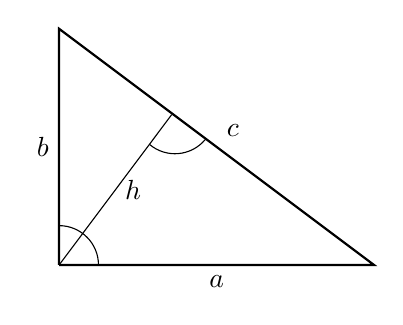
\begin{tikzpicture}
            \draw[thick] (0, 0) -- (4, 0) node[midway, below]{$a$} -- (0, 3) node[midway, above right]{$c$} -- (0, 0) node[midway, left]{$b$};
            \draw (0, 0) -- (1.43, 1.91) node[midway, right]{$h$};
            \draw (0.5, 0) arc (0:90:0.5);
            \draw (1.15, 1.53) arc (230:320:0.5);
          \end{tikzpicture}
        \end{center}
        \begin{gather}
          h = \sqrt{c_1\cdot c_2}\\
          s = \frac 12c\\
          r = \frac{a+b-c}{2}
        \end{gather}
      \subsubsection{Trójkąt równoboczny}
        \begin{center}
          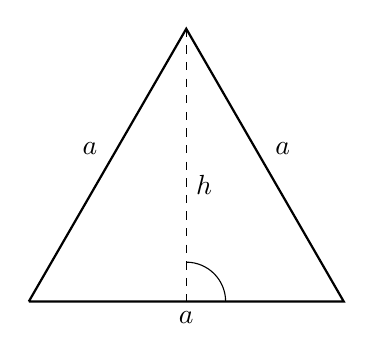
\begin{tikzpicture}
            \draw[thick] (0, 0) -- (4, 0) node[midway, below]{$a$} -- (2, 3.464) node[midway, above right]{$a$} -- (0, 0) node[midway, above left]{$a$};
            \draw[dashed] (2, 3.464) -- (2, 0) node[midway, below right]{$h$};
            \draw (2.5, 0) arc (0:90:0.5);
          \end{tikzpicture}
        \end{center}
        \begin{gather}
          h = \frac{a\sqrt3}{2}\\
          s = h\\
          r = \frac 13h = \frac{a\sqrt3}{6}\\
          r + R = h
        \end{gather}
    \subsubsection{Kwadrat}
      \begin{center}
        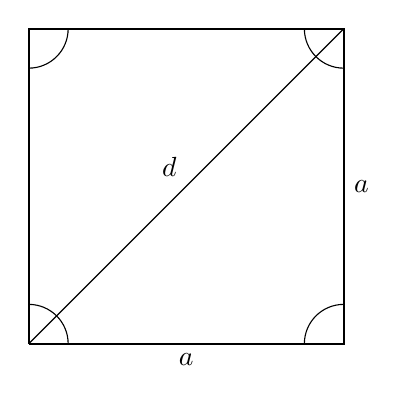
\begin{tikzpicture}
          \draw[thick] (0, 0) -- (4, 0) node[midway, below]{$a$} -- (4, 4) node[midway, right]{$a$} -- (0, 4) -- (0, 0);
          \draw (0, 0) -- (4, 4) node[midway, above left]{$d$};
          \draw (0.5, 0) arc (0:90:0.5);
          \draw (4, 0.5) arc (90:180:0.5);
          \draw (3.5, 4) arc (180:270:0.5);
          \draw (0, 3.5) arc (270:360:0.5);
        \end{tikzpicture}
      \end{center}
      \begin{gather}
        P = a^2 = \frac{d^2}{2}\\
        R = \frac 12d = \frac 12a\sqrt2\\
        r = \frac 12a
      \end{gather}
    \subsubsection{Prostokąt}
      \begin{center}
        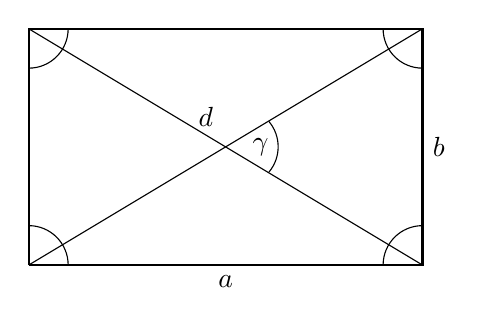
\begin{tikzpicture}
          \draw[thick] (0, 0) -- (5, 0) node[midway, below]{$a$} -- (5, 3) node[midway, right]{$b$} -- (0, 3) -- (0, 0);
          \draw (0, 0) -- (5, 3) node[midway, above left, xshift=-1, yshift=4]{$d$};
          \draw (0, 3) -- (5, 0);
          \draw (3.05, 1.18) arc (-40:40:0.5) node[midway, left]{$\gamma$};
          \draw (0.5, 0) arc (0:90:0.5);
          \draw (5, 0.5) arc (90:180:0.5);
          \draw (4.5, 3) arc (180:270:0.5);
          \draw (0, 2.5) arc (270:360:0.5);
        \end{tikzpicture}
      \end{center}
      \begin{align}
        &P = ab\\
        &P = \frac 12d^2\sin\gamma
      \end{align}
    \subsubsection{Romb}
      \begin{center}
        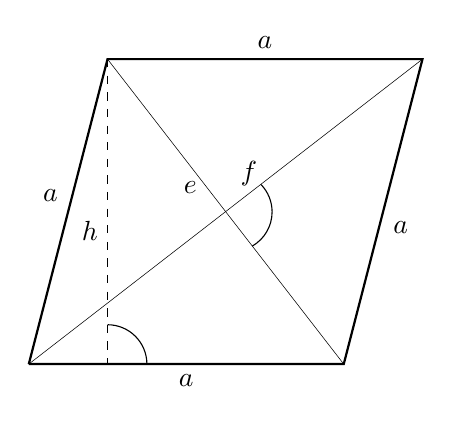
\begin{tikzpicture}
          \draw[thick] (0, 0) -- (4, 0) node[midway, below]{$a$} -- (5, 3.873) node[midway, below right]{$a$} -- (1, 3.873) node[midway, above]{$a$} -- (0, 0) node[midway, above left]{$a$};
          \draw[dashed] (1, 3.873) -- (1, 0) node[midway, below left]{$h$};
          \draw[very thin] (1, 3.873) -- (4, 0) node[midway, above left, xshift=-7, yshift=3]{$e$};
          \draw[very thin] (0, 0) -- (5, 3.873) node[midway, above right, xshift=2, yshift=6]{$f$};
          \draw (2.84, 1.5) arc (-60:44:0.5);
          \draw (1.5, 0) arc (0:90:0.5);
        \end{tikzpicture}
      \end{center}
      \begin{align}
        &P = ah\\
        &P = \frac{ef}{2}\\
        &P = a^2\sin\alpha
      \end{align}
    \subsubsection{Równoległobok}
      \begin{center}
        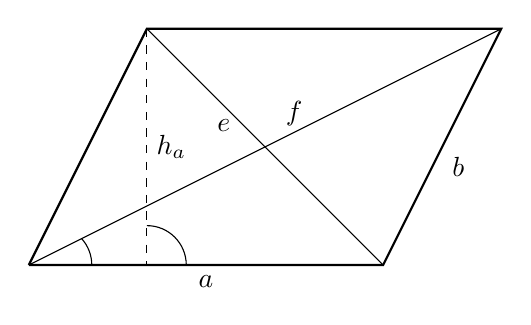
\begin{tikzpicture}
          \draw[thick] (0, 0) -- (4.5, 0) node[midway, below]{$a$} -- (6, 3) node[midway, below right]{$b$} -- (1.5, 3) -- (0, 0);
          \draw (0, 0) -- (6, 3) node[midway, above right, xshift=4, yshift=4]{$f$};
          \draw (1.5, 3) -- (4.5, 0) node[midway, above left, xshift=-9, yshift=2]{$e$};
          \draw[dashed] (1.5, 3) -- (1.5, 0) node[midway, right]{$h_a$};
          \draw (2, 0) arc (0:90:0.5);
          \draw (0.8, 0) arc (0:42:0.5);
        \end{tikzpicture}
      \end{center}
      \begin{align}
      &P = ah_a = bh_b\\
      &P = ab\sin\alpha
      \end{align}
    \subsubsection{Trapez}
      \begin{center}
        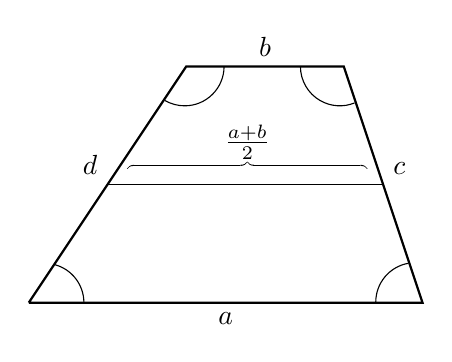
\begin{tikzpicture}
          \draw[thick] (0, 0) -- (5, 0) node[midway, below]{$a$} -- (4, 3) node[midway, above right]{$c$} -- (2, 3) node[midway, above]{$b$} -- (0, 0) node[midway, above left]{$d$};
          \draw (1, 1.5) -- (4.5, 1.5);
          \draw[decorate, decoration={calligraphic brace}] (1.25, 1.7) -- (4.3, 1.7) node[midway, above]{$\frac{a+b}{2}$};
          \draw (0.7, 0) arc (0:75:0.5);
          \draw (4.82, 0.5) arc (100:180:0.5);
          \draw (3.45, 3) arc (180:292:0.5);
          \draw (2.48, 3) arc (0:-120:0.5);
        \end{tikzpicture}
      \end{center}
      \begin{equation}
        P = \frac{(a+b)\cdot h}{2}
      \end{equation}
    \subsubsection{Trapez równoramienny}
      \begin{center}
        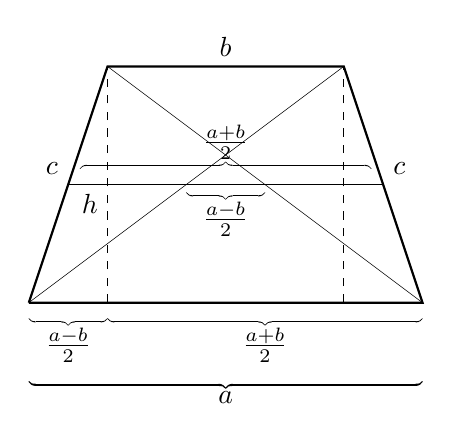
\begin{tikzpicture}
          \draw[thick] (0, 0) -- (5, 0) -- (4, 3) node[midway, above right]{$c$} -- (1, 3) node[midway, above] {$b$} -- (0, 0) node[midway, above left]{$c$};
          \draw[dashed] (1, 0) -- (1, 3) node[midway, below left] {$h$};
          \draw[dashed] (4, 0) -- (4, 3);
          \draw[very thin] (1, 3) -- (5, 0);
          \draw[very thin] (0, 0) -- (4, 3);
          \draw (0.5, 1.5) -- (4.5, 1.5);
          \draw[decorate, decoration={calligraphic brace}] (0.65, 1.7) -- (4.35, 1.7) node[midway, above]{$\frac{a+b}{2}$};
          \draw[decorate, decoration={calligraphic brace, mirror}] (2, 1.4) -- (3, 1.4) node[midway, below]{$\frac{a-b}{2}$};
          \draw[decorate, decoration={calligraphic brace, mirror}] (0, -0.2) -- (1, -0.2) node[midway, below]{$\frac{a-b}{2}$};
          \draw[decorate, decoration={calligraphic brace, mirror}] (1, -0.2) -- (5, -0.2) node[midway, below]{$\frac{a+b}{2}$};
          \draw[thick, decorate, decoration={calligraphic brace, mirror}] (0, -1) -- (5, -1) node[midway, below]{$a$};
        \end{tikzpicture}
      \end{center}
    \subsubsection{Deltoid}
      \begin{center}
        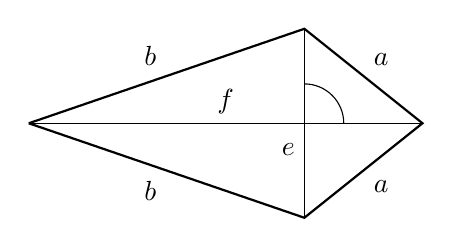
\begin{tikzpicture}
          \draw[thick] (0, 1.2) -- (3.5, 0) node[midway, below left]{$b$} -- (5, 1.2) node[midway, below right]{$a$} -- (3.5, 2.4) node[midway, above right]{$a$} -- (0, 1.2) node[midway, above left]{$b$};
          \draw[very thin] (3.5, 2.4) -- (3.5, 0) node[midway, below left, yshift=-4]{$e$};
          \draw[very thin] (0, 1.2) -- (5, 1.2) node[midway, above]{$f$};
          \draw (4, 1.2) arc (0:90:0.5);
        \end{tikzpicture}
      \end{center}
\end{document}
